\documentclass{article}
\usepackage[utf8]{inputenc}
\usepackage{graphicx}
\usepackage{amsmath}
\usepackage{float}

%User definded commands
\newcommand*\mean[1]{\bar{#1}}


\title{Project-thesis}
\author{Erik Rundhovde M\o renskog}
\date{September 2019}

\begin{document}

\maketitle

\section{Abstract}
This thesis will describe how to detect parameters in garbage 

Waste is a huge resource that is in large degrees wasted in todays society. In Norway 39\% is recycled, 57\% is burned for energy (Waste to energy or WtE) and 2\% goes into landfills \cite{EnvironmentGlance20152015} p.50. This thesis will look into one way of analyzing waste before burning. The idea is to use a spectrometer in the visible range combined with a camera to monitor the waste as it is inserted into the waste can. This will allow us to over time find parameters describing the waste, and possibly the objects the waste consists of. 


\section{Introduction}
The purpose of the system is to collect information about materials and objects in a manner similar to hyper-spectral imaging. Hyper-spectral imaging is extremely useful for classifying substances from a distance, but it is also very expensive. The setup being proposed in this paper is meant to be a cheaper replacement of the hyper-spectral one. 


\begin{figure}[H]
    \centering
    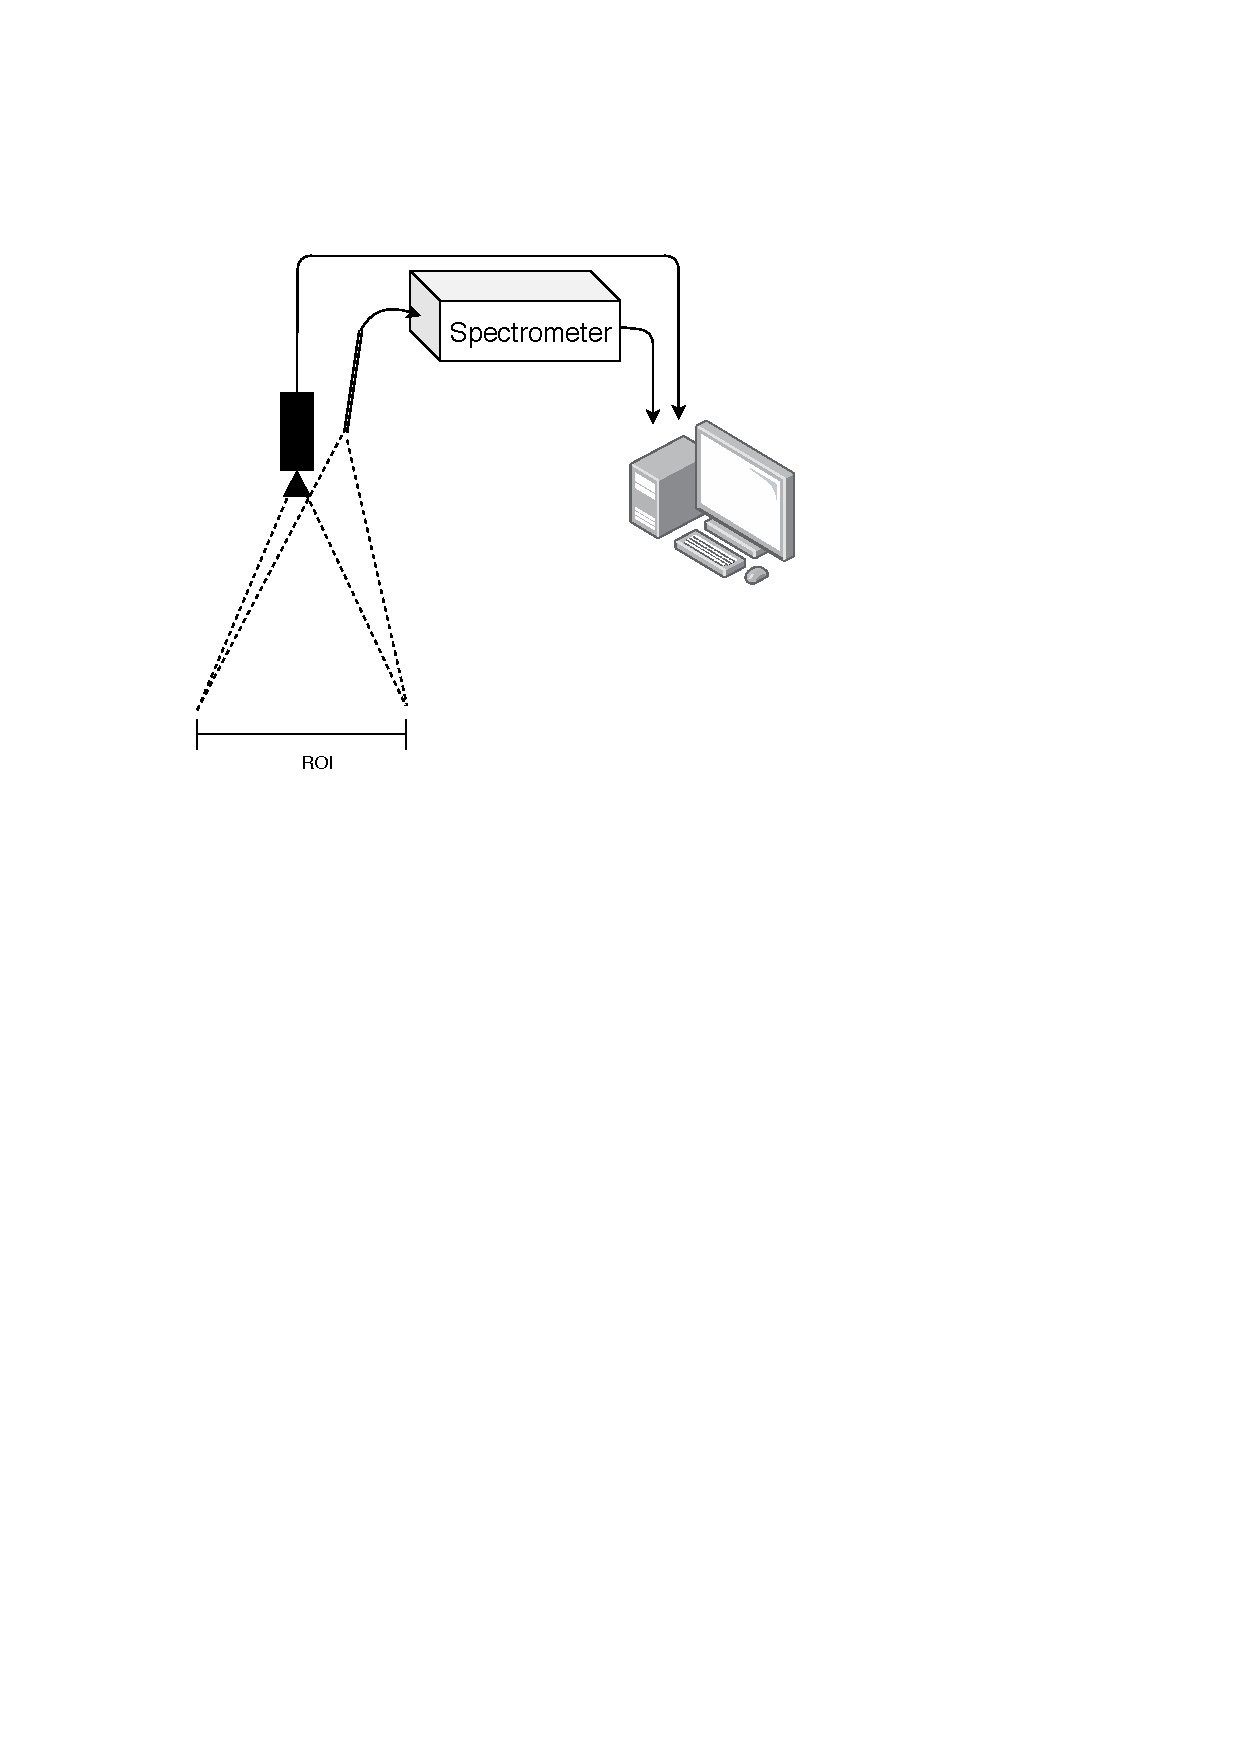
\includegraphics{figures/pt_setup.pdf}
    \caption{Measurement setup}
    \label{}
\end{figure}


\section{Theory}
Spectrometer is a widely used tool for analyzing substances. 

\subsection{Reflection}
Reflection of light describes the notion of light hitting materials and getting a change of path due to the exchange of energy with the material. 

\subsubsection{Specular}
\subsubsection{Diffusive}
\subsection{Relative reflection}


\subsection{Image}
Each image will be stored in a matrix where each element of the matrix is a vector described by (\ref{eq:vector_pixel_bgr}).
\begin{equation}
    \label{eq:vector_pixel_bgr}
    \vec{p}_{ij} = [B,G,R]
\end{equation} 
The vectors describes the color combination of each pixel, where each color; blue (B), green (G) and red (R) are unsigned integers. The matrix $A_{N\cdot M}$ is shown in (\ref{eq:image_matrix})

\begin{equation}
    \label{eq:image_matrix}
    A = A_{N\cdot M} =  
    \begin{bmatrix}
        \vec{p}_{11} & \vec{p}_{12} & \cdots & & \vec{p}_{1M}  \\
        \vec{p}_{21} & \ddots &        &       &                \\
        \vdots       &        &\vec{p}_{ij}&   & \vdots          \\
                     &        &        & \ddots&                  \\
        \vec{p}_{N1} &        &        &       & \vec{p}_{NM}  
    \end{bmatrix}
\end{equation}

An important equation later is the to take the spatial average of the matrix, this is done with (\ref{eq:spatial_sum}).

\begin{equation}
    \label{eq:spatial_sum}
    \mean{\vec{p}} = \frac{1}{N^2} \sum_{ij}^N \vec{p_{ij}}
\end{equation}


\subsection{Spectrum}
\label{sec:spectrum}

The spectrum read from the spectrometer is saved in a $C x 2$ matrix, where $C$ is the dataset length, the first column is the wavelength ($\lambda$) and the second column is the corresponding intensity (\ref{eq:intensity})
\begin{equation}
    \label{eq:intensity}
    I = I(\lambda)    
\end{equation}

\begin{equation}
    \label{eq:intensity_0_background}
    I_0 = I_0(\lambda)
\end{equation}

We will also define a value (\ref{eq:intensity_0_background}) which is $I$ for the special case where the spectrum is the background spectral response without any objects. From these definitions we define relative reflectance $RR$ (\ref{eq:relative_reflectance})

\begin{equation}
    \label{eq:relative_reflectance}
    RR = \frac{I}{I_0}
\end{equation}

We further introduce the notion of finding the spectrum corresponding to one color in the camera. Each pixel in the camera measures the light intensity for blue, green and red with a certain quantum efficiency (\ref{eq:quantum_efficiency}) given by the manufacturer. 

\begin{equation}
    \label{eq:quantum_efficiency}
    QE = QE(\lambda)    
\end{equation}

This value can theoretically be used to relate the relative picture values with the relative reflectance values. This would be a major advantage as it can give us an insight into the noise factor affecting the sensor fusion.  


\section{Method}
The idea is to use spectrometer methods to analyze images, this will open up for the opportunity to pre-process spectral and spatial data in the same way. We will then be able to compare the data directly. The point of this is to emulate a hyperspectral camera. 


\subsection{Correlating Spectrometer to Camera}
\label{sec:method_correlating_spectrum_to_camera}
To get an idea of how well calibrated the camera is to the spectrometer and vice versa I propose the following calculation: 
Take the spatial average across the image from the camera and divide it with the spectral average of the spectrometer. 



\subsection{Light}
Light is a crucial part of this project, as it is the source of input for both the camera and the spectrometer. It's also the link between the two sensors. The choosing of a sensor that can support both sensor types is therefore paramount. 

The characterization of the light source will be based on considerations from \cite{martinPracticalGuideMachine}, but also unfortunately be limited by available sources at the lab. This paper provides a longer checklist, that can be simplified greatly under the following conditions: Stationary objects,





\section{Results}

\subsection{Correlating Spectrometer to Camera}


\section{Conclusion}

It has proven very hard to correlate spectrometer and camera values that should be similar, even in ideal situations as in a dark lab.

\bibliographystyle{plain}
\bibliography{references.bib}
\end{document}